\documentclass{beamer}

\mode<presentation> {
	\usetheme{Darmstadt}
}

\usepackage{graphicx}
\usepackage{booktabs}
\usepackage{hyperref}
\usepackage{textcomp}
\usepackage{eurosym}
\usepackage{listings}
\usepackage{lstautogobble}
\usepackage{color}
\usepackage{ragged2e}
\usepackage{etoolbox}

\apptocmd{\frame}{}{\justifying}{} % Allow optional arguments after frame.

\setbeamertemplate{itemize item}[circle]

\definecolor{dkgreen}{rgb}{0,0.6,0}
\definecolor{gray}{rgb}{0.5,0.5,0.5}
\definecolor{mauve}{rgb}{0.58,0,0.82}
\definecolor{backcolour}{rgb}{0.95,0.95,0.92}

\lstset{frame=none,
  language=Java,
  aboveskip=0mm,
  belowskip=3mm,
  showstringspaces=false,
  columns=flexible,
  basicstyle=\small,
  numbers=left,
  numbersep=5pt,
  backgroundcolor=\color{backcolour},
  numberstyle=\tiny\color{gray},
  keywordstyle=\color{blue},
  commentstyle=\color{dkgreen},
  stringstyle=\color{mauve},
  breaklines=true,
  breakatwhitespace=true,
  tabsize=3,
  autogobble=true
}

%----------------------------------------------------------------------------------------
%	TITLE PAGE
%----------------------------------------------------------------------------------------

\title[Architecture Logicielle]{Architecture Logicielle}

\author{Lo\"{\i}c Ledoyen}
\institute[LEDOYEN EI] {
    \medskip
    \textit{ledoyen.esiea@gmail.com}
}
\date{\today}

\begin{document}

\begin{frame}
	\titlepage
\end{frame}

\begin{frame}
	\frametitle{Pourquoi l'architecture logicielle ?}
    
    \begin{itemize}
        \item maintenabilit\'{e} / \'{e}volutivit\'{e}
        \item testablit\'{e}
        \item fiabilit\'{e}
        \item scalabilit\'{e}
        \item s\'{e}curit\'{e}
        \item performance
    \end{itemize}
	~\\
    L{'}ordre de priorit\'{e} de ces objectifs doit \^{e}tre d\'{e}cid\'{e} par l{'}ensemble des acteurs du projet et r\'{e}ajust\'{e} autant que n\'{e}cessaire.
    \\~\\
    Il s{'}agit d{'}un \underline{\textbf{partenariat}}.
    \\~\\
    Le d\'{e}veloppeur met en \oe{}uvre les \textbf{principes d'architecture logicielle} pour r\'{e}pondre au mieux au \underline{\textbf{besoin}} du client.
\end{frame}

\begin{frame}
	\frametitle{Objectifs du cours}
    Conna\^{i}tre
	\begin{itemize}
        \item les bases de la programmation orient\'{e}e objet
        \item les outils de l'\'{e}cosyst\`{e}me du langage
        \item quelques patrons de conception
        \item quelques principes d'architecture \& m\'{e}thodologies de design
    \end{itemize}
    ~\\
    \begin{itemize}
    	\item Penser en terme de besoin pour arriver \`{a} la meilleur solution
        \item Bref, \^{e}tre un d\'{e}veloppeur
    \end{itemize}
\end{frame}

\begin{frame}
	\frametitle{Aller plus loin}

	YouTube - Devoxx FR
    \\~\\
	\url{http://www.codingthearchitecture.com/}
    \\~\\
	\url{http://martinfowler.com/}
    \\~\\
    \url{http://thinkbeforecoding.com/}
    
\end{frame}

\begin{frame}
	\frametitle{Contenu I}
	\tableofcontents[sections={1-2}]
\end{frame}

\begin{frame}
	\frametitle{Contenu II}
	\tableofcontents[sections={3-4}]
\end{frame}

\begin{frame}
	\frametitle{Contenu III}
	\tableofcontents[sections={5-6}]
\end{frame}

%----------------------------------------------------------------------------------------
%	INTRO
%----------------------------------------------------------------------------------------


\begin{frame}
	\frametitle{Introduction}

	Chacun son processus de cr\'{e}ation
    \\~\\
	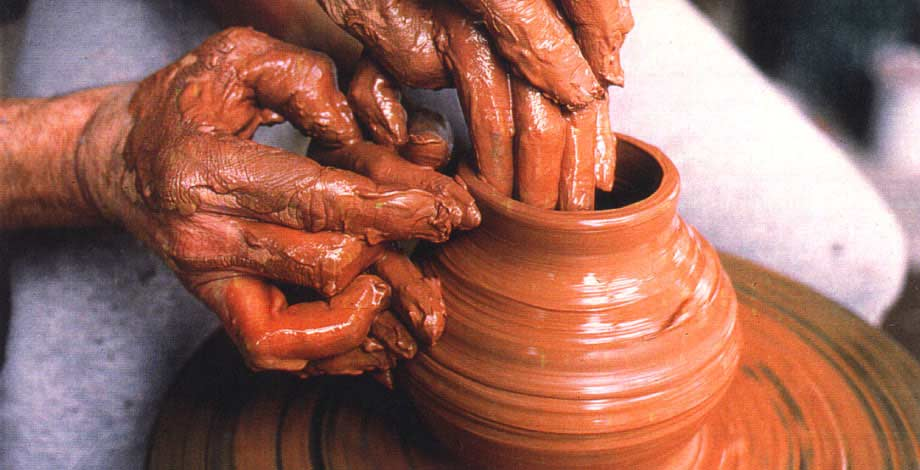
\includegraphics[width=7cm]{img/pottery.jpg}
    \\~\\
	Good programming is 99\% sweat and 1\% coffee.
\end{frame}

\section{Rappels de POO}

\begin{frame}
    \begin{center}
    \fontsize{48pt}{7.2}\selectfont
    Rappels de POO
    \end{center}
\end{frame}

\subsection{Objet}
\begin{frame}
\frametitle{Qu'est-ce qu'un objet ?}
Un \underline{objet} est une structure de \textbf{donn\'{e}es} qui r\'{e}pond \`{a} un ensemble de \textbf{messages}.
\\~\\
Les \underline{donn\'{e}es} sont appel\'{e}es \textbf{champs} (fields).
\\
Les \underline{messages} compris par un objet sont repr\'{e}sent\'{e}s par des fonctions de cet objet appel\'{e}es \textbf{m\'{e}thodes}.
\end{frame}

\begin{frame}[fragile]
\frametitle{Interface}
\begin{lstlisting}
public interface House {

	void addResident(Human resident);

	void removeResident(String name);

	int countResidents();
}
	\end{lstlisting}
\end{frame}

\begin{frame}[fragile]
\frametitle{Classe}
\begin{lstlisting}
import java.util.ArrayList;
import java.util.List;

public class CityHouse implements House {
	private final List<Human> residents = new ArrayList<>();

	public void addResident(Human resident) {
		if(!residents.contains(resident) {
			residents.add(resident);
		}
	}
	public void removeResident(String name) {
		residents.removeIf(h -> h.getName().equals(name));
	}
	public int countResidents() {
    	return residents.size();
    }
}
	\end{lstlisting}
\end{frame}

\begin{frame}[fragile]
\frametitle{Instance}
\begin{lstlisting}
public class HouseApplication {
	public static void main(String[] args) {
		House _21_jump_street = new CityHouse();

		_21_jump_street.addResident(new Human("Channing Tatum"));
		_21_jump_street.addResident(new Human("Jonah Hill"));

		System.out.println("Number of residents: " + _21_jump_street.countResidents()); // 2

		_21_jump_street.addResident(new Human("Jonah Hill"));

		System.out.println("Number of residents: " + _21_jump_street.countResidents()); // 2
	}
}
	\end{lstlisting}
\end{frame}

\subsection{S O L I D}

\begin{frame}
	\frametitle{S O L I D}
	\begin{itemize}
    	\item \textbf{S}ingle responsibility: une seule responsabilit\'{e} par classe
		\item \textbf{O}pen/Close: ouvert \`{a} la composition, ferm\'{e} \`{a} la modification
		\item \textbf{Liskov} substitution: substitution par un sous-type sans modification de la coh\'{e}rence
		\item \textbf{I}nterface segregation: une interface (contrat) diff\'{e}rente par client
		\item \textbf{D}ependency inversion: travailler avec la forme la plus abstraite d\'{}un objet (une interface en g\'{e}n\'{e}ral)
    \end{itemize}
    ~\\
    La programmation orient\'{e}e objet n'est r\'{e}ellement int\'{e}ressante qu'en mettant en \oe{}uvre les principes \textbf{S O L I D}.
\end{frame}

\begin{frame}[fragile]
	\frametitle{S O L I D: exemple I (L \& S)}
	\begin{lstlisting}
public interface Logger {
	void log(Level level, String message);
}
	\end{lstlisting}
    \begin{lstlisting}
public class ConsoleLogger implements Logger {
	public void log(Level level, String message) {
		System.out.prinln("[" + level + "] " + message);
	}
}
	\end{lstlisting}
    \begin{lstlisting}[basicstyle=\tiny]
public class FileLogger implements Logger {
	...
    public void log(Level level, String message) {
        try {
            Files.write(path, ("[" + level + "] " + message + "\n").getBytes(), APPEND, CREATE);
        } catch (IOException e) {
            throw new RuntimeException("Cannot write log message to file [" + path + "]", e);
        }
    }
}
	\end{lstlisting}
\end{frame}

\begin{frame}[fragile]
	\frametitle{S O L I D: exemple II (O \& D)}
	\begin{lstlisting}
import java.util.Arrays;

public class CompositeLogger implements Logger {

	private Iterable<Logger> delegates;

	public CompositeLogger(Logger... loggers) {
		this.delegates = Arrays.asList(loggers);
	}

	public void log(Level level, String message) {
		delegates.forEach(l -> l.log(level, message));
	}
}
	\end{lstlisting}
\end{frame}

\begin{frame}[fragile]
	\frametitle{S O L I D: exemple III (usage)}
	\begin{lstlisting}[basicstyle=\tiny]
import java.io.IOException;
import java.net.InetSocketAddress;
import java.net.Socket;

public class MyApplication {

	private static final Logger LOGGER = LoggerFactory.getLogger();

	public static void main(String[] args) {
		LOGGER.log(Level.INFO, "Application starts");

		String hostname = "google.com";
		int port = 80;
		int connectionTimeout = 2000; // in ms

		try (Socket socket = new Socket()) {
			socket.connect(new InetSocketAddress(hostname, port), connectionTimeout);
			LOGGER.log(Level.INFO, "Successfully connected to " + hostname);
		} catch (IOException e) {
			LOGGER.log(Level.ERROR, "Unable to connect to " + hostname + ": " + e.getMessage());
		}

		LOGGER.log(Level.INFO, "Application stops");
	}
}
	\end{lstlisting}
\end{frame}

\subsection{Thread}

\begin{frame}
	\frametitle{Qu'est-ce qu'un thread ?}
	Un \textbf{thread} est un fil d'ex\'{e}cution repr\'{e}sentant une t\^{a}che \`{a} effectuer.
    \\~\\
    La notion de thread est n\'{e}cessaire pour mod\'{e}liser des t\^{a}ches \`{a} r\'{e}aliser en parall\`{e}le.
    \begin{itemize}
    	\item un thread n\'{}est pas li\'{e} \`{a} un processeur
		\item il peut donc y en avoir plus que de processeurs (c\oe{}urs)
        \item un thread a \textit{globalement} deux \'{e}tats:
        \begin{itemize}
        	\item consommant du CPU
            \item attendant une notification
        \end{itemize}
        \item ex\'{e}cuter plusieurs threads sur un m\^{e}me processeur (c\oe{}ur) est co\^{u}teux
    \end{itemize}
    ~\\
    
\includegraphics[width=1cm]{img/karadoc.png}
    \begin{quote}
    \`{A} utiliser en toute technique d'arrosage donc
    \end{quote}
\end{frame}

\begin{frame}[fragile]
	\frametitle{Thread: Patron Object Pool}
    Il est possible d'utiliser la classe {\lstinline[basicstyle=\ttfamily\color{blue}]|java.lang.Thread|} afin de lancer directement un thread.
    \\~\\
    % Malformul\'{e}
    Cependant la fa\c{c}on la plus commune de g\'{e}rer ses threads depuis \textbf{Java 5} est d'utiliser le patron de conception \textbf{Object Pool} disponible via l'interface {\lstinline[basicstyle=\ttfamily\color{blue}]|java.util.concurrent.ExecutorService|}.
    \\~
    \begin{lstlisting}[basicstyle=\tiny]
import java.util.concurrent.*;

...
	public static void main(String[] args) throws InterruptedException {
		Runnable task1 = () -> System.out.println("Hello");
		Runnable task2 = () -> System.out.println("World");

		ExecutorService pool = Executors.newFixedThreadPool(2);

		try {
			pool.submit(task1);
			pool.submit(task2);
			pool.awaitTermination(100L, TimeUnit.MILLISECONDS);
		} finally {
			pool.shutdown();
		}
	}
	\end{lstlisting}
\end{frame}

\begin{frame}[fragile]
	\frametitle{Thread Safety}
    \begin{lstlisting}
private int counter = 0;

public int increment() {
    int tmp = counter;
    tmp = tmp + 1;
    counter = tmp;
    return tmp;
}
	\end{lstlisting}
    Solutions:
    \begin{itemize}
    	\item verrous ({\lstinline[basicstyle=\ttfamily\color{blue}]|synchronized|})
        \item types atomiques ({\lstinline[basicstyle=\ttfamily\color{blue}\small]|AtomicBoolean|}, etc.)
    \end{itemize}
    
    Il existe \'{e}galement le mot-cl\'{e} {\lstinline[basicstyle=\ttfamily\color{blue}]|volatile|} permettant d'obtenir la valeur "\`{a} jour" d\'{}une variable et non la valeur dans le cache du processeur.
    \\~\\
    {\lstinline[basicstyle=\color{red}]|Attention|} cependant, {\lstinline[basicstyle=\ttfamily\color{blue}]|volatile|} ne garantie pas l\'{}atomicit\'{e} des op\'{e}rations effectu\'{e}es sur la variable.
\end{frame}

\begin{frame}[fragile]
	\frametitle{Outillage pour manipuler des threads}    
    Il existe plein de bonnes choses dans le \textit{package} {\lstinline[basicstyle=\ttfamily\color{blue}]|java.util.concurrent|} permettant de contr\^{o}ler des threads
    \begin{itemize}
    	\item {\lstinline[basicstyle=\ttfamily\color{blue}]|Executors|}
    	\item {\lstinline[basicstyle=\ttfamily\color{blue}]|Semaphore|}
    	\item {\lstinline[basicstyle=\ttfamily\color{blue}]|CyclicBarrier|}
        \item {\lstinline[basicstyle=\ttfamily\color{blue}]|CompletableFuture|}
        \item ...
    \end{itemize}
    ~\\
    Il existe aussi des librairies d\'{e}di\'{e}es au \textit{flow control}
    \begin{itemize}
    	\item RxJava
    	\item Spring\'{}s{\lstinline[basicstyle=\ttfamily\color{blue}]| @Async|}
        \item librairies autours de NIO2 ({\lstinline[basicstyle=\ttfamily\color{blue}]|java.nio.*|})
        \item ...
    \end{itemize}
\end{frame}

\subsection{Collections}
\begin{frame}[fragile]
	\frametitle{Collections}
    Une collection est un ensemble d\'{}objet de m\^{e}me type.
    \\~\\
    % Ce sont presque des objets. Ils ne peuvent pas \^{e}tre \'{e}tendus, n'ont pas de nom de classe, sont utilis\'{e}s avec une syntaxe qui leur est propre, et ils h\'{e}ritent des m\'{e}thodes de la classe Object, notamment toString()
    Contrairement \`{a} un tableau, la taille d'une collection peut changer par l'ajout ou la suppression d\'{}\'{e}l\'{e}ments.
    \\~\\
    Une {\lstinline[basicstyle=\ttfamily\color{blue}]|Collection|} est {\lstinline[basicstyle=\ttfamily\color{blue}]|Iterable|}.
    \\~\\
    Cela signifie qu'elle doit renvoyer un objet {\lstinline[basicstyle=\ttfamily\color{blue}]|Iterator|}.
    \\~\\
    Un {\lstinline[basicstyle=\ttfamily\color{blue}]|Iterator|} va permettre d\'{}it\'{e}rer sur les \'{e}l\'{e}ments contenus dans la collection.
\end{frame}

\begin{frame}[fragile]
	\frametitle{Relations entre les classes de Collection}
    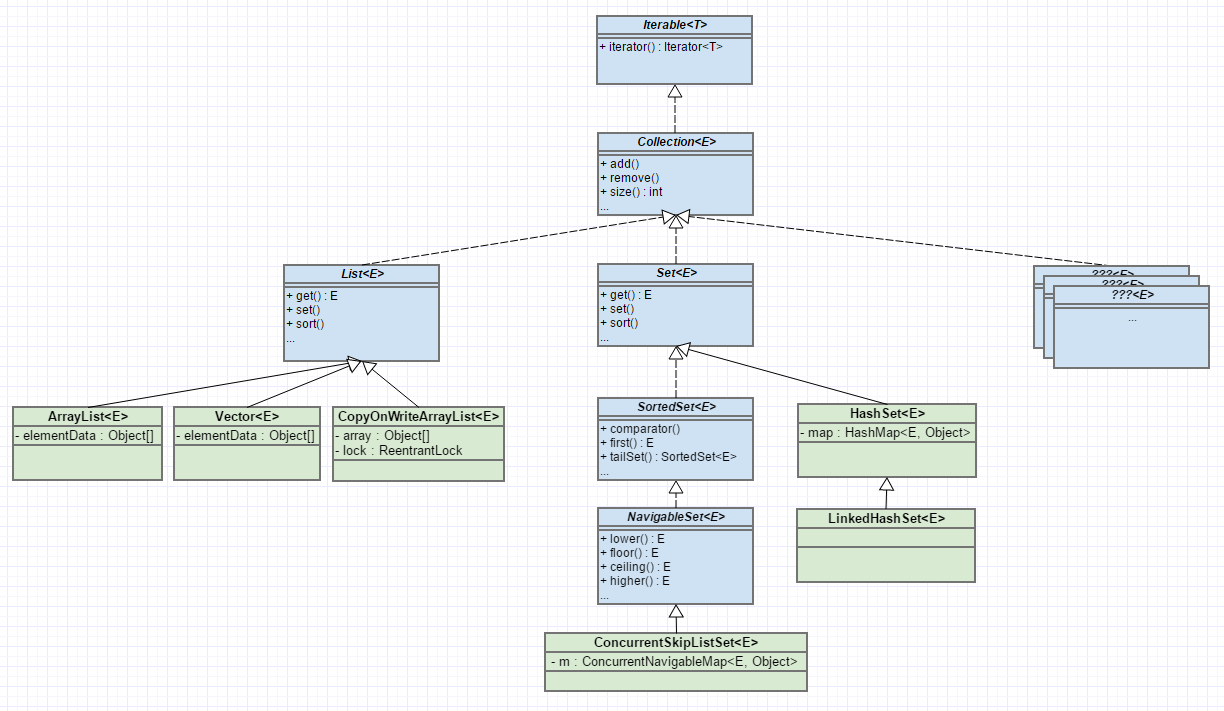
\includegraphics[width=11cm]{img/collections.png}
\end{frame}

\begin{frame}[fragile]
	\frametitle{Collections en Java}
    \begin{itemize}
      \item Une collection est un type \textit{g\'{e}n\'{e}rique}
      \item Le type d\'{}objet contenu est indiqu\'{e} entre chevron
      \item L\'{}interface de plus haut niveau est utilis\'{e}e pour les types des variables et des param\`{e}tres
    \end{itemize}
    ~\\
    \begin{lstlisting}
private final List<Human> humans = new ArrayList<Human>();

public boolean isAnyNameContained(Set<String> names) {
	return humans.stream()
		.filter(h -> names.contains(h.name))
		.findAny()
		.isPresent();
}
	\end{lstlisting}
    Ici le param\`{e}tre {\lstinline[basicstyle=\ttfamily\color{blue}]|Set<String> names|} impose \`{a} l'utilisateur un argument sans doublon.
\end{frame}


\section{\'{E}cosyst\`{e}me du d\'{e}veloppeur}

\begin{frame}
    \begin{center}
    \fontsize{48pt}{7.2}\selectfont
    \'{E}cosyst\`{e}me du d\'{e}veloppeur
    \end{center}
\end{frame}

\subsection{Syst\`{e}me de gestion de version}
\begin{frame}
	\frametitle{SCM: Source Code Management}
    Qu\'{}ils soient centralis\'{e}s ou d\'{e}centralis\'{e}s, il existe plusieurs syst\`{e}mes (CSV, SVN, Mercurial, GIT, etc.).
    \\~\\
    Ces syst\`{e}mes fonctionnent par diff\'{e}rentiel (patch) afin de permettre de restaurer une version pr\'{e}c\'{e}dente ou encore de travailler sur une version parall\`{e}le qui pourra plus tard \^{e}tre r\'{e}-incorpor\'{e}e dans la version principale.
    \\~\\
    On parle de
    \begin{itemize}
      \item \textbf{branch} pour d\'{e}crire un fil de modification
      \item \textbf{tag} pour identifier une version bien particuli\`{e}re
      \item \textbf{merge}  lors de la r\'{e}union de deux branches
      \item \textbf{checkout} pour r\'{e}cup\'{e}rer la version d\'{}un d\'{e}p\^{o}t
      \item \textbf{commit} pour envoyer des modifications sur un d\'{e}p\^{o}t
    \end{itemize}
\end{frame}

\begin{frame}
	\frametitle{SCM: Source Code Management}
    ~\\
	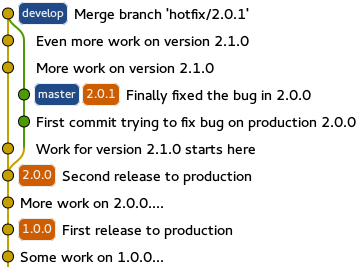
\includegraphics[width=8cm]{img/git_sample.png}
    ~\\
\end{frame}

\subsection{Moteur de construction}
\begin{frame}
	\frametitle{Build automation tool}
Du plus vieux (\textbf{make}) aux plus utilis\'{e}s dans le monde Java (\textbf{Maven}, \textbf{Graddle}), ces outils permettent de g\'{e}rer
~
\begin{itemize}
      \item les d\'{e}pendances utilis\'{e}es
      \item le lancement des tests
      \item la construction d'un projet (packaging)
      \item son rapport au syst\`{e}me de gestion de version
      \item son cycle de vie dans le syst\`{e}me d'int\'{e}gration continue
      \item son param\`{e}trage
      \item la g\'{e}n\'{e}ration de la documentation
    \end{itemize}
\end{frame}

\begin{frame}
	\frametitle{Maven I}
	\textbf{Maven} propose de baser l\'{}organisation du projet suivant des conventions plut\^{o}t que la description des t\^{a}ches n\'{e}cessaires \`{a} sa gestion.
	\\~\\
    Ainsi un projet \textbf{Maven} doit avoir cette structure
    \\
    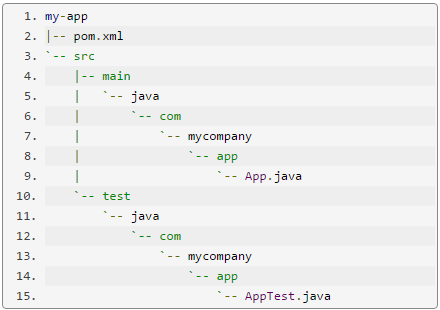
\includegraphics[width=7cm]{img/maven_structure.png}
\end{frame}

\begin{frame}
	\frametitle{Maven II}
    Par d\'{e}faut Maven utilise un cycle de vie permettant \`{a} la grande majorit\'{e} des projets d\'{}\^{e}tre construit sans configuration.
    \\~\\
    \url{https://maven.apache.org/guides/introduction/introduction-to-the-lifecycle.html}
    \\~\\
    Les principales \textbf{phases} sont
    \begin{itemize}
      \item \textbf{clean} : nettoie les fichiers compil\'{e}s ou g\'{e}n\'{e}r\'{e}s
      \item \textbf{compile} : compile les sources \textit{principales (main)}
      \item \textbf{test-compile} : compile les sources de \textit{test}
      \item \textbf{test} : lance les tests
      \item \textbf{package} : construit le binaire, \textbf{jar} par d\'{e}faut
      \item \textbf{install} : place le binaire dans le d\'{e}p\^{o}t Maven local
      \item \textbf{deploy} : place le binaire dans un d\'{e}p\^{o}t Maven distant
      \item \textbf{site} : g\'{e}n\'{e}re la documentation
    \end{itemize}
\end{frame}

\begin{frame}
	\frametitle{Maven III}
    Chaque phase est associable \`{a} un ou des \underline{\textbf{plugins}}, ce qui rend Maven tr\'{e}s extensible.
    \\~\\
    Des plugins sont fournis directement par Maven, comme le \textbf{maven-clean-plugin}.
    \\~\\
    D\'{}autre sont cr\'{e}\'{e}s par la communaut\'{e} sans voir besoin de modifier l\'{}outil :
    \begin{itemize}
      \item \textbf{cukedoctor-maven-plugin} : produit une version HTML du r\'{e}sultat des tests Cucumber
      \item \textbf{sonar-maven-plugin} : analyse le code avec diff\'{e}rents outils (PMD, Checkstyle, JaCoCo, etc.) et pousse les r\'{e}sultats dans un serveur Sonar
      \item etc.
    \end{itemize}
\end{frame}

\begin{frame}[fragile]
	\frametitle{Maven}
    \begin{center}
    \fontsize{48pt}{7.2}\selectfont
    D\'{e}mo
    \end{center}
    \begin{center}
    (Cr\'{e}ation d'un projet, g\'{e}n\'{e}ration de la documentation)
    \\~\\
    \begin{lstlisting}
mvn archetype:generate
	-DarchetypeArtifactId=maven-archetype-quickstart
    -DgroupId=fr.esiea
    -DartifactId=fruit-basket

mvn site
		\end{lstlisting} 
    \end{center}
\end{frame}

\begin{frame}
	\frametitle{Maven : phases \& plugins du packaging jar}
    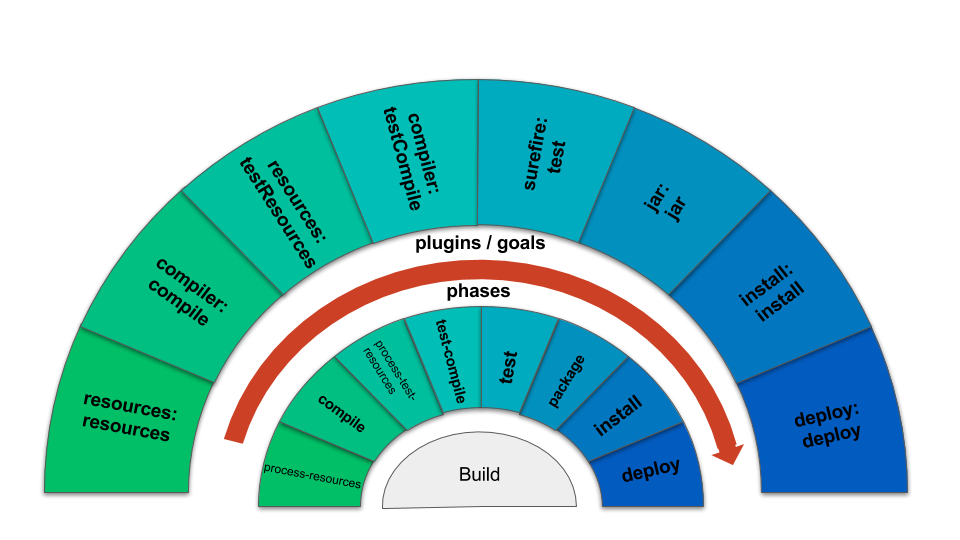
\includegraphics[width=11cm]{img/maven_circle.png}
\end{frame}

\subsection{D\'ep\^{o}t}
\begin{frame}
	\frametitle{Repository Manager}
    Il en existe plusieurs (Nexus, Artifactory, etc.) , c\'{}est l\'{}endroit o\`{u} vont tous les binaires.
    \\~\\
    Aussi bien ceux produits par l\'{}int\'{e}gration continue de votre projet que les d\'{e}pendances que votre projet utilise.
    \\~\\
    Pour cela, les diff\'{e}rents outils int\'{e}ragissant avec le d\'{e}p\^{o}t fonctionnent avec les conventions de nommage de Maven
    
\begin{itemize}
	\item Le \textbf{G.A.V} (\textbf{G}roupId, \textbf{A}rtifactId, \textbf{V}ersion) identifie un binaire
    \item La structure d'un d\'ep\^{o}t est identique \`{a} celle du d\'ep\^{o}t local
    \begin{itemize}
    	\item \textbf{\texttildelow{}/.m2/repository/}junit/junit/4.12/junit-4.12.jar
        \item \textbf{http://central.maven.org/maven2/}junit/junit/4.12/junit-4.12.jar
    \end{itemize}
\end{itemize}
\end{frame}

\subsection{IDE (Integrated development environment)}
\begin{frame}
	\frametitle{IDE}
    Il en existe plusieurs (Eclipse, IntelliJ, etc.), c\'{}est l\'{}outil qui aide le d\'{e}veloppeur \`{a} taper du code plus vite et en faisant moins d'erreur.
    \\~\\
    Pour cela, ces outils int\`{e}grent des raccourcis claviers aidant \`{a} la cr\'{e}ation rapide de fichier, de structure, au lancement de t\^{a}che r\'{e}p\'{e}titives, \`{a} la visualisation de la documentation.
    \\~\\
    Il est important pour un d\'{e}veloppeur d\'{}\^{e}tre \`{a} l'aise avec un IDE afin de produire rapidement des POC ou encore de s'attaquer \`{a} de gros \textit{refactoring} sans crainte d'erreur ou de r\'{e}gressions.
\end{frame}

\subsection{Plugins}
\begin{frame}
	\frametitle{Plugins}
    Un plugin (extension ou encore greffon) peut \^{e}tre vu comme l'inverse d'un framework en ce sens qu'un plugin va \^{e}tre appel\'{e} par du code et non le contraire.
    \\~\\
    La plupart des outils de d\'{e}veloppement offre une API permettant le d\'{e}veloppement de plugins.
    \\~\\
    C'est le cas de GIT, Maven, Eclipse, ou encore de Jenkins (int\'{e}gration continue).
    \\~\\
    \underline{Minimalistes} dans leurs concepts de base, ces outils autorisent \underline{l'ajout de} \underline{fonctionnalit\'{e}s}.
    \\~\\
    \textbf{L'ouverture \`{a} la composition} est un principe important de l'architecture logicielle ici mis en exemple.
\end{frame}

\subsection{Tests}
\begin{frame}
	\frametitle{Tests I}
    Les tests servent trois objectifs:
\begin{itemize}
    \item rassurer le d\'{e}veloppeur sur la bonne fonction de son code, maintenant et dans le futur
    \item rassurer l\'{}\'{e}quipe projet
    \item montrer comment le code produit doit ou peut \^{e}tre utilis\'{e}
\end{itemize}
~\\
On trouve commun\'{e}ment le d\'{e}coupage suivant:
\begin{itemize}
    \item Unit Test: teste un fragment de code, en g\'{e}n\'{e}ral une seule m\'{e}thode ($<$300ms)
    \item Integration Test: teste l'interfacage avec un framework, un autre applicatif, etc. ($<$1min)
    \item Acceptance Test: teste une fonctionnalit\'{e} compl\`{e}te du point de vue m\'{e}tier
\end{itemize}
\end{frame}

\begin{frame}
	\frametitle{Tests II}
    Chacun de ces types de test est int\'{e}ressant et se focalise sur des objectifs diff\'{e}rents.
    \\~\\
    Si des tests doivent \^{e}tre longs, il faut qu'ils soient pertinents.
    \\~\\
    De cette mani\`{e}re la boucle de r\'{e}tro-action est la plus courte possible.
    \\~\\
    Il est donc n\'{e}cessaire de mat\'{e}rialiser une diff\'{e}rence entre chaque type de test.
	\\~\\
	Maven propose une convention : *Test.java et *IT.java
    \\~\\
    Configuration par d\'{e}faut des plugins \textbf{maven-surefire-plugin} et \textbf{maven-failsafe-plugin} li\'{e}s aux phases \textbf{test} et \textbf{integration-test}.
\end{frame}

\begin{frame}
	\frametitle{Tests III}
    Pour les AT, il peut \^{e}tre n\'{e}cessaire d'utiliser une solution ext\'{e}rieure au moteur de construction (Fitnesse, Robot Framework, Concordion, etc.).
    \\~\\
    En effet, ce genre de test s'ex\'{e}cute sur une application \textit{d\'{e}ploy\'{e}e} et non avant la construction du binaire.
    \\~\\
    Contrairement aux deux premiers types de test, ces tests doivent pouvoir \^{e}tre lus et compris par des intervenants du projet non-d\'{e}veloppeur (notamment les garants fonctionnels du projet: PO, MOA, etc.).
    \\~\\
    C'est pourquoi des outils tels que \textbf{Cucumber} sont utilis\'{e}s, afin de pouvoir r\'{e}diger ses tests dans un langage naturel (Anglais, Francais, etc.) plut\^{o}t que dans un langage technique (Java, Python, etc.)
\end{frame}

\begin{frame}
	\frametitle{Tests}
    \begin{center}
    \fontsize{48pt}{7.2}\selectfont
    D\'{e}mo
    \end{center}
    \begin{center}
    (Le panier de fruit en TDD)
    \end{center}
\end{frame}

\subsection{Profiler, flamegraph et APM}
\begin{frame}
	\frametitle{Profiler, flamegraph et APM I}
    Il peut \^{e}tre n\'{e}cessaire d'aller au del\`{a} du debug, pour voir le temps pass\'{e} dans chaque m\'{e}thodes, ou d\'{e}celer une fuite m\'{e}moire.
    \\~\\
    Pour cela, il existe diff\'{e}rents outils qui permettent d'observer dans le d\'{e}tail le comportement d'une application pendant son ex\'{e}cution : les \textbf{profilers}.
    \\~\\
    Pour descendre encore, le \textbf{flamegraph} permet de faire la corr\'{e}lation entre les m\'{e}thodes (telles qu'observ\'{e}es avec un profiler) et l'ex\'{e}cution du code de l'\textit{OS} afin de voir ce qui consomme le plus de CPU.
    \\~\\
    Enfin il existe \'{e}galement des solutions d'\textbf{A}pplication \textbf{P}erformance \textbf{M}onitoring \& Management qui permettent de voir l'activit\'{e} d'un syst\`{e}me complet (load-balancer, application, BDD, etc.), de d\'{e}celer les erreurs et de \textit{zoomer} sur l\'{}\'{e}l\'{e}ment probl\'{e}matique.    
\end{frame}

\begin{frame}
	\frametitle{Profiler, flamegraph et APM II}
    A l'exception du flamegraph et de quelques profilers (type hprof), la plupart de ces solutions sont tr\`{e}s pratiques, mais... payantes (AppDynamics, NewRelic, Introscope, etc.).
    \\~\\
    Il est \`{a} noter que toutes ces solutions souffrent du m\^{e}me probl\`{e}me : la sur-consommation CPU (\textit{overhead}).
    \\~\\
    Cette sur-consommation peut \^{e}tre un probl\`{e}me dans un syst\`{e}me o\`{u} les performances sont importantes.
    \\~\\ Seuls les APM peuvent vraiment \^{e}tre utilis\'{e}s sur un syst\`{e}me en production car ils utilisent un \'{e}chantillonnage intelligent permettant de ne pas trop d\'{e}grader les performances tout en conservant une bonne pr\'{e}cision.
\end{frame}


\section{\'{E}cosyst\`{e}me de l'\'{e}quipe de d\'{e}veloppement}

\begin{frame}
    \begin{center}
    \fontsize{48pt}{7.2}\selectfont
    \'{E}cosyst\`{e}me de l'\'{e}quipe de d\'{e}veloppement
    \end{center}
\end{frame}

\subsection{Tests}
\begin{frame}
	\frametitle{Tests... again}
    Comme on l'a vu, les tests servent \`{a} \textbf{rassurer l\'{}\'{e}quipe projet}.
    \\~\\
    Cela signifie que les membres de l\'{}\'{e}quipe vont chercher dans les tests accompagnant un d\'{e}veloppement :
    \begin{itemize}
        \item une mise \`{a} plat du besoin
        \item une documentation du code
        \item une s\'{e}curit\'{e} pour de futurs changements (refactoring)
        \item une assurance que la section test\'{e}e fonctionnera en \textbf{\textit{Production}}
    \end{itemize}
	~\\
	Il faudra donc \^{e}tre vigilant \`{a} deux points cl\'{e}s:
    \begin{itemize}
        \item la couverture de code
        \item les assertions
    \end{itemize}
\end{frame}

\subsection{Relecture de code}
\begin{frame}
	\frametitle{Relecture de code I}
    La relecture, ou revue de code est l'action de faire valider son code par un autre membre de l\'{}\'{e}quipe.
    \\~\\
    La revue s'attarde \`{a} travailler sur un morceau de code \textbf{\textit{restreint}} correspondant \`{a} une \'{e}volution ou une correction.
    \\~\\
    Elle peut \^{e}tre formelle (obligatoire) au travers d'outils tels que Gerrit, ou informelle en travaillant \`{a} 2 ou plus sur un m\^{e}me clavier (pair-programming).
    \\~\\
    La revue de code est un des outils de l\'{}\'{e}quipe pour faire fasse \`{a} plusieurs probl\'{e}matiques :
    \begin{itemize}
        \item le passage de connaissance
        \item la d\'{e}tection de bug
        \item le respect de la \textbf{\textit{vision technologique}} du projet
    \end{itemize}
\end{frame}

\begin{frame}
	\frametitle{Relecture de code II}
    Afin de rendre le travail plus simple et d'y passer le moins de temps possible, il est pr\'{e}f\'{e}rable de proposer \`{a} l\'{}\'{e}quipe des morceaux de code (branche, PR ou juste commit) les plus petits possibles.
    \\~\\
    La revue de code est un outil tr\`{e}s puissant, mais il est facile d'y perdre beaucoup de temps.
    \\~\\
    Il existe quelques r\`{e}gles simples mais c'est \`{a} chaque \'{e}quipe de trouver sa mani\`{e}re de proc\'{e}der :
    \begin{itemize}
        \item le code est la responsabilit\'{e} de l\'{}\'{e}quipe, \'{e}viter de le personnifier (\textbf{le} code plut\^{o}t que \textbf{ton}/\textbf{son} code)
        \item couper court aux d\'{e}bats d'opinions, s'il y a d\'{e}bat, les arguments doivent \^{e}tre objectifs
        \item privil\'{e}gier la parole \`{a} l\'{}\'{e}change formel (chat, mail, etc.)
    \end{itemize}
\end{frame}

\subsection{Pourquoi les patrons de conception ?}
\begin{frame}
	\frametitle{Design Patterns I}
    Les patrons de conceptions \underline{proposent} des solutions adapt\'{e}es \`{a} des besoins \textit{standards}.
    \\~\\
    Il est int\'{e}ressant d'en comprendre quelques-uns afin de confronter les solutions qu'ils proposent \`{a} une approche na\"{i}ve.
    \\~\\
    Il n'est cependant pas recommand\'{e} de commencer \`{a} coder en s'appuyant directement sur des \textit{designs patterns}.
    \\~\\
    On parle dans ce cas d\'{}\'{e}mergence plut\^{o}t que de \textit{Big Design Up Front}.
    \\~\\
    Pour cela il est important de se focaliser sur le m\'{e}tier de l'application, \textbf{puis} d'identifier les sections qui sont susceptibles d'\^{e}tre impl\'{e}ment\'{e}es gr\^{a}ce \`{a} des design patterns.
\end{frame}

\begin{frame}
	\frametitle{Design Patterns II}
    Les \textit{patrons de conceptions} sont un outil de l\'{}\'{e}quipe permettant de \underline{converger} vers une solution standard.
    \\~\\
    Attention toutefois \`{a} ce que la solution soit adapt\'{e}e au besoin.
\end{frame}

\subsection{Int\'{e}gration continue}
\begin{frame}
	\frametitle{Int\'{e}gration continue}
    L'int\'{e}gration continue consiste \`{a} lancer r\'{e}guli\`{e}rement, voir \`{a} chaque changement de la base de code, certaines taches du cycle de vie du projet, notamment:
    \begin{itemize}
        \item la compilation
        \item les tests (unitaires et d'int\'{e}gration)
        \item la cr\'{e}ation de binaires \textit{snapshot}
        \item l'analyse de la qualit\'{e} du code
        \item la g\'{e}n\'{e}ration de la documentation
    \end{itemize}
    ~\\
    Cela permet \`{a} l\'{}\'{e}quipe d'avoir un retour rapide sur l'avancement du projet ainsi qu'une centralisation des taches r\'{e}p\'{e}titives comme le d\'{e}ploiement sur divers environnements ou encore le lancement des tests d'acceptation.
\end{frame}

\subsection{Mesure de la qualit\'{e} du code}
\begin{frame}
	\frametitle{Qualit\'{e} du code}
    Il existe de nombreux outils d'analyse de la qualit\'{e} du code.
    Cela comprend
    \begin{itemize}
        \item l'analyse statique qui s'attache \`{a} v\'{e}rifier le code source. Dans l'\'{e}cosyst\`{e}me Java il en existe plusieurs : checkstyle, findbugs, PMD, etc.
        \item l'analyse dynamique qui v\'{e}rifie le comportement au moment de l'ex\'{e}cution. C'est ce type d'analyse qui permet de conna\^{i}tre la portion de code couverte par les diff\'{e}rents types de tests (JaCoCo, etc.)
    \end{itemize}
    ~\\
    Ces analyses peuvent \^{e}tre regroup\'{e}s dans un outil central, aliment\'{e} via l'int\'{e}gration continue.
    \\~\\
    Ainsi l'\'{e}quipe peut d\'{e}finir les r\`{e}gles/conventions qu'elle souhaite suivre et v\'{e}rifier leur respect tout au long de la vie du projet.
\end{frame}

\begin{frame}
	\frametitle{CI \& Quality}
    \begin{center}
    \fontsize{48pt}{7.2}\selectfont
    D\'{e}mo
    \end{center}
    \begin{center}
    (Jenkins \& Sonar)
    \end{center}
\end{frame}

\subsection{Supervision}
\begin{frame}
	\frametitle{Supervision I}
La supervision est un outil important de l'\'{e}quipe qui permet de
	\begin{itemize}
        \item comprendre le comportement d'une application en condition r\'{e}elle
        \item \^{e}tre alert\'{e} lorsqu'un probl\`{e}me appara\^{i}t
    \end{itemize}

    ~\\
    La supervision peut \^{e}tre con\c{c}ue en r\'{e}pondant \`{a} 3 questions :
    \begin{itemize}
    	\item Quels sont les comportements du syst\`{e}mes que l'on souhaite identifier comme probl\'{e}matiques (service indisponible, utilisation anormale, etc.) ?
        \item Quels comportements du syst\`{e}mes souhaite-t-on comprendre (coups de b\'{e}liers, interruption de services externes, etc.) ?
        \item O\`{u} placer les sondes qui remonterons les informations n\'{e}cessaires ?
    \end{itemize}
\end{frame}

\begin{frame}[fragile]
	\frametitle{Supervision II}
    On peut utiliser, entre autres, les stacks suivantes:
    \\~\\
    Logstash $\longrightarrow$ ElasticSearch $\longrightarrow$ Kibana / ElastAlert
    \begin{itemize}
      \item[] + centralisation et analyse des logs
      \item[] + (plugin timelion pour les s\'{e}ries temporelles)
      \item[] - peu adapt\'{e} aux s\'{e}ries temporelles
      \item[] - alertes non int\'{e}gr\'{e}es aux dashboards
    \end{itemize}
    ~\\
    collectd / sql-to-graphite $\longrightarrow$ Graphite $\longrightarrow$ Grafana
	\begin{itemize}
      \item[] + La taille de la BDD (carbon) est d\'{e}finie \`{a} l'avance
      \item[] + adapt\'{e} aux s\'{e}ries temporelles
      \item[] - uniquement aux s\'{e}ries temporelles
    \end{itemize}
\end{frame}

\begin{frame}[fragile]
	\frametitle{Supervision III}
Dans l'\'{e}cosyst\`{e}me Java, les m\'{e}triques peuvent \^{e}tre produites en utilisant l'API JMX (Java Management Extensions).
    \\~\\
    Cette API permet (entre autre) d'exposer des m\'{e}triques num\'{e}riques, notamment gr\^{a}ce \`{a} des librairies comme \textit{metrics} de Dropwizard.
    \\~\\
        \begin{lstlisting}
	@RequestMapping("/create_user")
	Customer createUser(@RequestParam("firstName") String firstName, @RequestParam("lastName") String lastName) {
		final Timer.Context context = timer.time(); // starts the timer
		try {
			Customer newCustomer = repository.create(firstName, lastName)
			LOGGER.info("Saved new " + newCustomer);
			return newCustomer;
		} finally {
			context.stop(); // stops and compute results
		}
	}
	\end{lstlisting}
\end{frame}

\begin{frame}
	\frametitle{Supervision}
    \begin{center}
    \fontsize{48pt}{7.2}\selectfont
    D\'{e}mo
    \end{center}
    \begin{center}
    (Serveur REST \& JConsole)
    \end{center}
\end{frame}


\section{D\'{e}marrer un projet en \'{e}quipe}

\begin{frame}
    \begin{center}
    \fontsize{48pt}{7.2}\selectfont
    D\'{e}marrer un projet en \'{e}quipe
    \end{center}
\end{frame}

\subsection{K I S S}
\begin{frame}[fragile]
	\frametitle{K I S S}
	\textbf{Keep It Stupid Simple}, un principe de base valant \`{a} tous les niveaux, du code \`{a} l'organisation de l'\'{e}quipe en passant par l'architecture du projet.
    \\~\\    
	\begin{lstlisting}
private static int sumAbsoluteElements(ArrayList<Integer> list) {
	int sum = 0;

	for (Iterator<Integer> iter = list.iterator(); iter.hasNext();) {
		Integer value = iter.next();
		if (value > 0) {
			sum += value;
		} else {
			sum -= value;
		}
	}

	return sum;
}
	\end{lstlisting}
\end{frame}

\begin{frame}[fragile]
	\frametitle{K I S S}
    
    La simplicit\'{e} est la sophistication supr\^{e}me. (L\'{e}onard De Vinci)
    \\~\\
	\begin{lstlisting}
public int absoluteSum(Collection<Integer> numbers) {
	return numbers.stream().mapToInt(Math::abs).sum();
}
	\end{lstlisting}
\end{frame}


\subsection{C4}

\begin{frame}
	\frametitle{C4 I}
    
    \textbf{C4} est une approche pour concevoir un syst\`{e}me informatique sans compliquer inutilement l'architecture.
    \\~\\
    Pour ce faire, il est n\'{e}cessaire d'\'{e}tablir un ensemble de termes et d'abstractions avec lesquels tous les intervenants du projet pourront se \textbf{comprendre}.
    \\~\\
    C'est une \'{e}tape cruciale, qui permet d'\'{e}viter par la suite d'avoir des incompr\'{e}hension entre les diff\'{e}rents corps de m\'{e}tier (fonctionnels, d\'{e}veloppeurs, int\'{e}grateurs, etc.).
    \\~\\
    Ce sont ces \'{e}l\'{e}ments qui permettront de construire les diagrammes qui seront \`{a} la base du projet.
\end{frame}

\begin{frame}
	\frametitle{C4 II}
    
    Avec cette base, les intervenants peuvent construire le \textbf{diagramme de contexte}.
    \\~\\
    Ce diagramme permet de comprendre les principales fonctionnalit\'{e}s du syst\`{e}me sans afficher comment le syst\`{e}me est organis\'{e}.
    \\~\\
    Le syst\`{e}me est repr\'{e}sent\'{e} par une unique forme (boite noire) qui sera en interaction avec des personnes ou d'autres syst\`{e}mes.
    \\~\\
    Les d\'{e}tails (technologies, protocoles, etc.) n'ont pas d'importance dans ce diagramme, il doit pouvoir \^{e}tre compris par des intervenants non-techniques.
\end{frame}

\begin{frame}
	\frametitle{C4 III}

    \textbf{Exemple de diagramme de contexte}\\
    \centerline{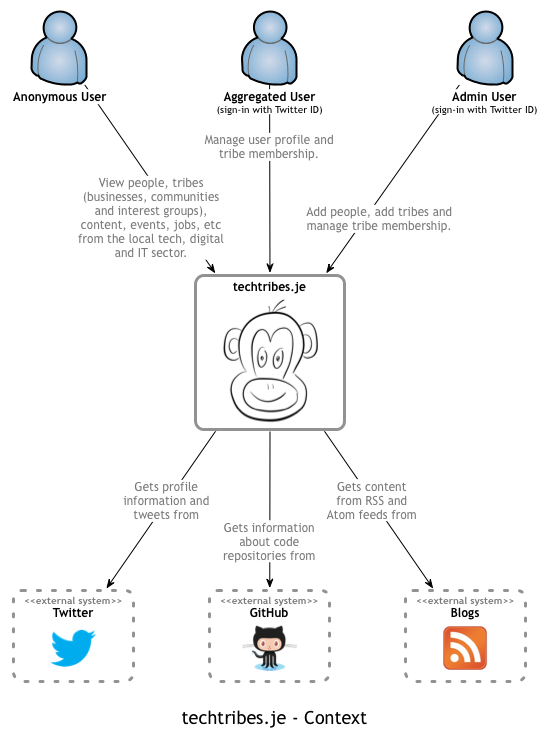
\includegraphics[width=5cm]{img/context_diagram.png}}
\end{frame}

\begin{frame}
	\frametitle{C4 IV}
    
    Une fois les fonctionnalit\'{e}s du syst\`{e}mes acquises, on peut \textit{zoomer} d'un cran avec le \textbf{diagramme de \textit{conteneurs}}.
    \\~\\
    On entend par \textit{conteneur} tout syst\`{e}me qui peut h\'{e}berger du code ou des donn\'{e}es (application, base de donn\'{e}es, broker, etc.).
    \\~\\
    Ce diagramme va refl\'{e}ter l'architecture du syst\`{e}me et permettre de visualiser comment les responsabilit\'{e}s sont r\'{e}parties parmi les diff\'{e}rentes briques logicielles.
    \\~\\
    Ici peuvent \^{e}tre repr\'{e}sent\'{e}s
    \begin{itemize}
    	\item la \textbf{s\'{e}curit\'{e}} : zones r\'{e}seau, flux chiffr\'{e}s, tra\c{c}abilit\'{e}, etc.
        \item la \textbf{scalabilit\'{e}} : load-balancers, (SPOF), etc.
        \item la \textbf{fiabilit\'{e}} : sauvegarde, r\'{e}plication, etc
        \item la \textbf{supervision} : sondes, bases, IHM, etc.
    \end{itemize}
\end{frame}

\begin{frame}
	\frametitle{C4 V}

    \textbf{Exemple de diagramme de conteneurs}\\
    \centerline{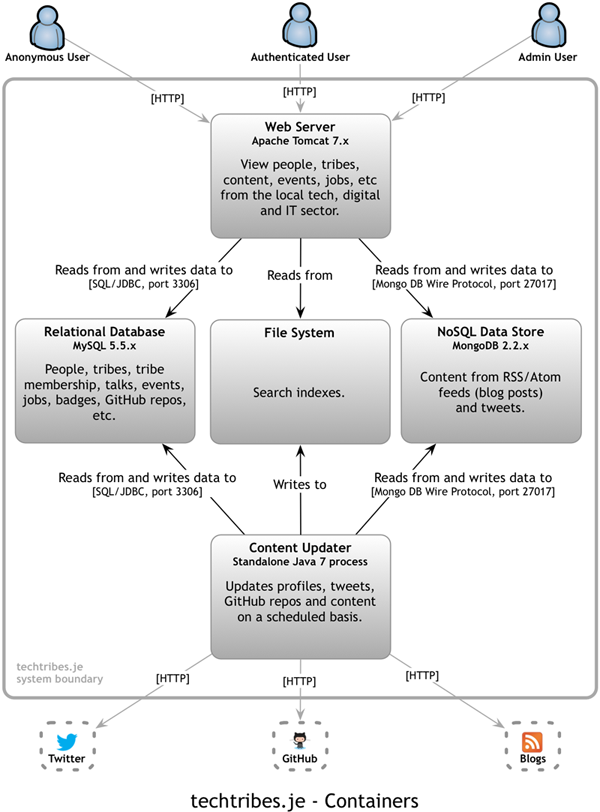
\includegraphics[width=5cm]{img/container_diagram.png}}
\end{frame}

\begin{frame}
	\frametitle{C4 VI}
    
    On peut \`{a} nouveau \textit{zoomer} sur chacun des conteneurs gr\^{a}ce au \textbf{diagramme de composants}.
    \\~\\
    Ce diagramme d\'{e}taille ce dont est compos\'{e} un conteneur, avec un d\'{e}coupage possible par
    \begin{itemize}
    	\item fonctionnalit\'{e} transverse
        \item service m\'{e}tier
        \item workflow
    \end{itemize}
    ~\\
    Un composant a donc une identit\'{e} logique, une \underline{responsabilit\'{e}} et interagit avec d'autres composants.
    \\~\\
    Sont habituellement consign\'{e}s les d\'{e}tails d'impl\'{e}mentation et choix technologiques car ce sch\'{e}ma peut \^{e}tre la documentation la plus d\'{e}taill\'{e}e d'un projet.
\end{frame}

\begin{frame}
	\frametitle{C4 VII}

    \textbf{Exemple de diagramme de composants}\\
    \centerline{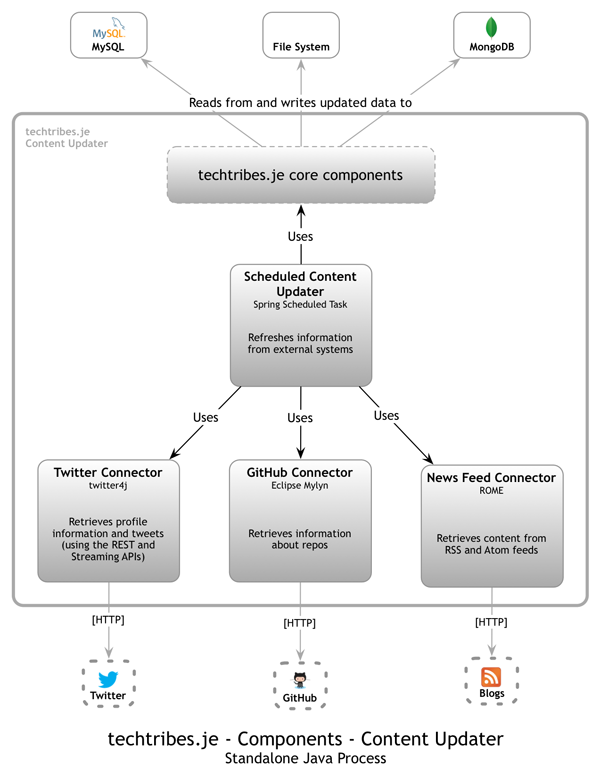
\includegraphics[width=5cm]{img/component_diagram.png}}
\end{frame}

\begin{frame}
	\frametitle{C4 VIII}
    Si n\'{e}cessaire, il est possible de descendre au classique \textbf{diagramme UML de classes}.
    \\~\\
    Ce diagramme est rarement utile si les besoins sont clairs, et les responsabilit\'{e}s bien r\'{e}parties.
    \\~\\
    Cependant, pour mod\'{e}liser un comportement complexe, ce sch\'{e}ma peut mettre en lumi\`{e}re une interaction complexe entre plusieurs objets.
\end{frame}

\begin{frame}
	\frametitle{C4 IX}

    \textbf{Exemple de diagramme de classes}\\
    \centerline{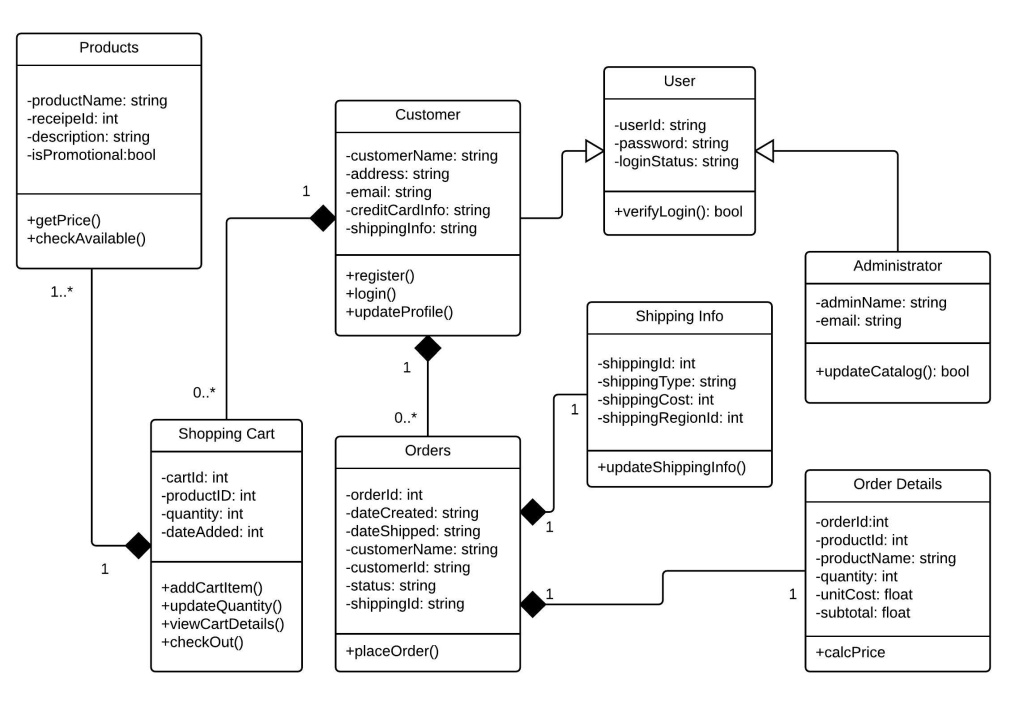
\includegraphics[width=8cm]{img/class_diagram.jpg}}
\end{frame}

\subsection{Architecture Hexagonale}
\begin{frame}
	\frametitle{Architecture Hexagonale I}

    Il s'agit d'un type d'architecture o\`u le code m\'etier est s\'epar\'e des sp\'ecifit\'es techniques.\\
	~\\
	Cette approche rejoint le DDD (Domain Design Development) en ce sens que l'effort est concentr\'e dans un premier temps sur la mod\'elisation du domaine avec le vocabulaire de l'entreprise.\\
	~\\
	Ainsi isol\'e des probl\'ematiques techniques, le code m\'etier est simple \`a lire, \`a tester, \`a faire \'evoluer.\\
	~\\
	Dans un second temps des adapteurs sont d\'evelopp\'es pour connecter le code m\'etier avec le monde ext\'erieur (web-service, base de donn\'ees, etc.)\\
	~\\
	\textbf{\color{red}{Le code m\'etier ne doit avoir aucune d\'ependance sur les adapteurs.}}
\end{frame}

\begin{frame}
	\frametitle{Architecture Hexagonale II}

    \centerline{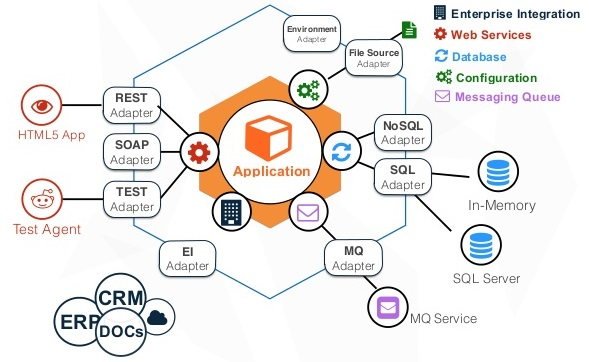
\includegraphics[width=10cm]{img/hexagonal-architecture.jpg}}
\end{frame}

\begin{frame}
	\frametitle{Architecture Hexagonale III}

    On parle de
	\begin{itemize}
    	\item \textbf{\color{blue}{API}} : le code m\'etier qui est appel\'e par des adapteurs
        \item \textbf{\color{blue}{SPI}} : le code m\'etier qui appelle des adapteurs
    \end{itemize}
	
	\textbf{\color{blue}{API}} et \textbf{\color{blue}{SPI}} sont une s\'erie d'interface qui permettent le d\'ecouplage entre les diff\'erentes parties du code.\\
	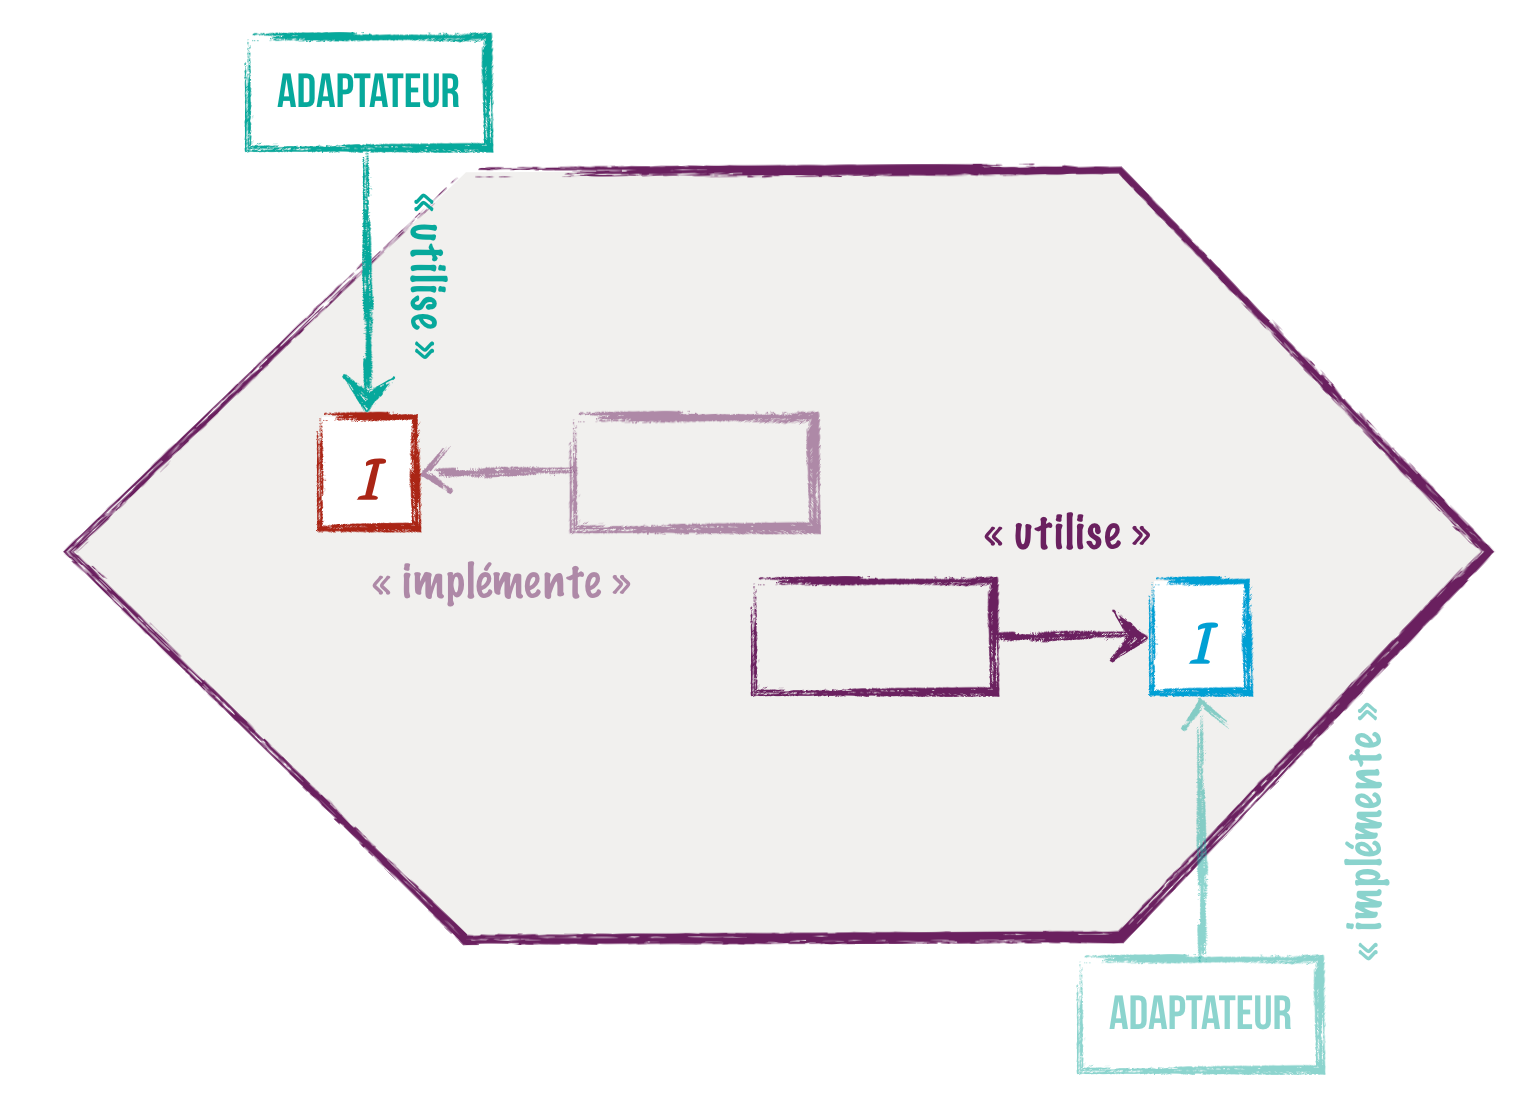
\includegraphics[width=6cm]{img/api_vs_spi1.png}
\end{frame}

\begin{frame}
	\frametitle{Architecture Hexagonale IV}

    Ce \textit{pattern d'architecture} permet \`a faible cout de :
	\begin{itemize}
    	\item faciliter le test des r\`egles m\'etier
        \item simplifier le remplacement d'un adapteur par un autre (changement de protocol par ex.)
		\item am\'eliorer la lisibilit\'e du code
    \end{itemize}
	
	~\\
	En outre le code m\'etier \'etant fid\`ele au domaine, c'est une bonne base pour la documentation vivante (Living Documentation).
\end{frame}

\subsection{D\'{e}veloppement pilot\'{e} par les tests (TDD, BDD)}
\begin{frame}
	\frametitle{TDD}
    Le d\'{e}veloppement pilot\'{e} par les tests (\textbf{T}est-\textbf{D}riven \textbf{D}evelopment) consiste \`{a} coder les tests avant l'application.
    \\~\\
    On entend par test principalement les tests unitaires, mais le principe peut \^{e}tre \'{e}tendu \`{a} tous les types, y compris les tests de recette automatis\'{e}s (AT).
    \\~\\
    Afin que le code compile, il est souvent n\'{e}cessaire de coder le squelette du programme, c'est-\`{a}-dire une m\'{e}thode vide.
    \\~\\
    C'est un processus it\'{e}ratif, il n'est pas n\'{e}cessaire de coder tous les tests du premier coup.
    \\~\\
    Tester un code revient \`{a} le brancher dans un autre composant, le composant d\'{e}velopp\'{e} est donc \underline{test\'{e} et facilement utilisable}.
\end{frame}

\begin{frame}
	\frametitle{BDD I}
    Le BDD (\textbf{B}ehavior-\textbf{D}riven \textbf{D}evelopment) est quasiment la m\^{e}me chose que le TDD.
    \\~\\
    La subtilit\'{e} est qu'on ne teste plus une application, mais qu'on d\'{e}finit son comportement.
    \\~\\
    Pour cela le BDD propose d'\'{e}crire en langage naturel, avec une s\'{e}mantique chronologique :
    \begin{itemize}
    	\item Given : les condition initiales
        \item When : \'{e}l\'{e}ment d\'{e}clencheur (unique)
        \item Then : v\'{e}rifications
    \end{itemize}
	~\\
	L'avantage du BDD est de fournir des cahiers de tests lisibles par tous et faciles \`{a} \'{e}crire pour un d\'{e}veloppeur.
\end{frame}

\begin{frame}[fragile]
	\frametitle{BDD II}
    La structure des outils de BDD associant des phrases (patterns) \`{a} du code (m\'{e}thodes), permet naturellement la composition.
    \\~\\
    \begin{lstlisting}[basicstyle=\tiny]
Feature: Owner service

Scenario: Owner list is empty on startup
  Given database is empty
  When an HTTP GET request is made on resource /owner/list
  Then the HTTP response code should be OK
  Then the HTTP response body should be []

Scenario: Owner creation
  Given database is empty
  When an HTTP POST request is made on resource /owner with content
    """
      {
      	"firstName": "Steeve",
      	"lastName": "Jobs"
      }
    """
  Then the HTTP response code should be CREATED
  And an HTTP GET request on resource /owner/list should respond status 200 with body matching
  | Expression                             | Expected result |
  | $[?(@.firstName == 'Steeve')].lastName | Jobs            |
	\end{lstlisting}
\end{frame}

\subsection{Des logs pour tous}
\begin{frame}
	\frametitle{Des logs pour tous I}

    Les logs sont indispensables pour comprendre un dysfonctionnement, elles servent essentiellement de contexte d'ex\'{e}cution.
    \\~\\
    Les logs peuvent \^{e}tre lues par :
    \begin{itemize}
    	\item les d\'{e}veloppeurs
        \item les int\'{e}grateurs
        \item les testeurs (recette)
        \item les administrateurs syst\`{e}me
    \end{itemize}
    ~\\
    C'est pourquoi il est important que les logs soient claires et apportent le maximum d'informations possibles.
    \\~\\
    Pour cela on \'{e}vite les logs visuelles ou de debug.
\end{frame}

\begin{frame}[fragile]
	\frametitle{Des logs pour tous II}

    \begin{lstlisting}[basicstyle=\tiny]
2017-02-04 22:33:12 [main] com.github.lolo.projet.DatabaseService l.74 #################
2017-02-04 22:33:12 [main] com.github.lolo.projet.DatabaseService l.75 START
2017-02-04 22:33:12 [main] com.github.lolo.projet.DatabaseService l.93 STOP in 17ms
2017-02-04 22:33:12 [main] com.github.lolo.projet.DatabaseService l.94 #################
2017-02-04 22:33:12 [main] com.github.lolo.projet.DatabaseService l.124 java.sql.SQLIntegrityConstraintViolationException
	at org.h2.message.DbException.getJdbcSQLException(DbException.java:345)
	at org.h2.message.DbException.get(DbException.java:179)
	at org.h2.message.DbException.get(DbException.java:155)
	at org.h2.command.CommandContainer.update(CommandContainer.java:98)
	at org.h2.command.Command.executeUpdate(Command.java:258)
	at org.h2.jdbc.JdbcPreparedStatement.execute(JdbcPreparedStatement.java:201)
	... 50 more
    \end{lstlisting}
    ~\\
    \'{E}viter les informations inutiles.\\
    Exprimer le \textbf{maximum} en un \textbf{minimum de lignes}.
    \\~\\
    \begin{lstlisting}[basicstyle=\tiny]
2017-02-04 22:33:12.332 INFO  c.g.l.p.UserService.create [Joshua] [Bloch] Save successful
2017-02-04 22:33:12.758 INFO  c.g.l.p.UserService.create [Doug] [Lea] Save successful
2017-02-04 22:33:12.964 ERROR c.g.l.p.UserService.create [James] [Gosling] Save KO: already exists
    \end{lstlisting}
\end{frame}

\begin{frame}[fragile]
	\frametitle{Des logs pour tous III}

    Pour faciliter la cr\'{e}ation de logs, il existe de nombreuses libs.
    \\~\\
    Elles se retrouvent pour la plupart autour de la structure suivante:
     \begin{itemize}
    	\item \textbf{Logger} : recueille les informations \'{e}mises \`{a} divers endroits de l'application
        \item \textbf{Appender} : agr\`{e}ge et sauvegarde les informations (dans un fichier, dans une base, vers un broker, etc.)
    \end{itemize}
    ~\\
    On configure donc habituellement
    \begin{itemize}
    	\item le niveau de verbosit\'{e} (importance) de chaque \textbf{logger}
        \item le format et la destination d'un \textbf{appender}
    \end{itemize}
    
\end{frame}

\begin{frame}[fragile]
	\frametitle{Des logs pour tous IV}

    En utilisant le pattern MDC (\textbf{M}apped \textbf{D}iagnostic \textbf{C}ontext), il est possible de transporter des informations contextuelles : 
    \begin{itemize}
    	\item ID de corr\'{e}lation
        \item param\`{e}tre de service standard
        \item origine d'une requ\^{e}te
        \item ID de run (pour un batch par ex.)
        \item etc.
    \end{itemize}
    ~\\
    Ainsi sans alourdir les appels aux m\'{e}thodes ou aux loggers, les informations sont stock\'{e}es dans le contexte du Thread traitant la requ\^{e}te.
    \\~\\
    Ces informations peuvent ensuite \^{e}tre retrouv\'{e}es directement dans la configuration des appenders.
\end{frame}

\begin{frame}[fragile]
	\frametitle{Des logs pour tous V}

    \begin{lstlisting}[basicstyle=\tiny]
public void onMessage(Message message) {
    MDC.put("ID_MESSAGE", message.getId());
    try {
        service.save(message.getContent());
        LOGGER.info("Save successful");
    } catch(InvalidMessageException e) {
        LOGGER.error("Save KO: " + e.getMessage());
    }
}
    \end{lstlisting}
    ~\\
    \begin{lstlisting}[basicstyle=\tiny]
	<appender name="STDOUT" class="ch.qos.logback.core.ConsoleAppender">
		<encoder>
      		<pattern>%d{yyyy-MM-dd HH:mm:ss} %-5level %logger{36} [%X{ID_MESSAGE}] %msg%n</pattern>
    	</encoder>
	</appender>
    \end{lstlisting}
    ~\\
    \begin{lstlisting}[basicstyle=\tiny]
2017-02-04 22:33:12 INFO  c.g.l.p.MessageListener [78456878] Save successful
2017-02-04 22:33:14 ERROR c.g.l.p.MessageListener [78456879] Save KO: Unable to parse JSON invalid character { at pos 61.
2017-02-04 22:33:12 INFO  c.g.l.p.MessageListener [78456880] Save successful
    \end{lstlisting}
\end{frame}

\begin{frame}[fragile]
	\frametitle{Logs \& Librairies}

    Dans beaucoup de langages, il n'y a pas de standard et les librairies et frameworks ont chacun leur solution de logging.
    \\~\\
    De mani\`{e}re \`{a} centraliser les logs capt\'{e}es par les diff\'{e}rentes librairies de logging, on peut utiliser des \textbf{\textit{bridges}}.
    \\~\\
    Il va s'agir d'intercepter les appels aux diff\'{e}rentes solutions et de les rediriger vers une unique librairie.
    \\~\\
    En Java, SLF4J propose une solution double :
    \begin{itemize}
    	\item une couche d'abstraction permettant de changer d'impl\'{e}mentation sans changer de code
        \item des bridges pour rediriger les logs des autres librairies de log
    \end{itemize}  
\end{frame}

\begin{frame}
	\frametitle{SLF4J}

    \centerline{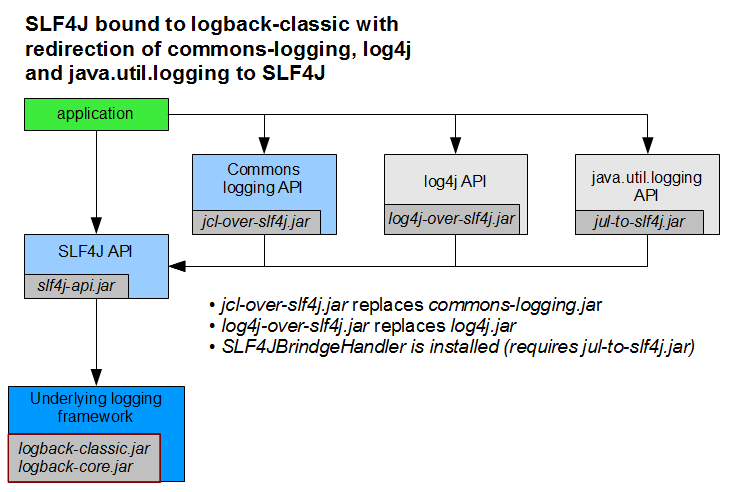
\includegraphics[width=11cm]{img/slf4j.png}}
\end{frame}

\begin{frame}
    \begin{center}
    \fontsize{48pt}{7.2}\selectfont
    D\'{e}mo
    \end{center}
    \begin{center}
    (SLF4J)
    \end{center}
\end{frame}


\section{Coder en \'{e}quipe}

\begin{frame}
    \begin{center}
    \fontsize{48pt}{7.2}\selectfont
    Coder en \'{e}quipe
    \end{center}
\end{frame}

\begin{frame}
	\frametitle{Coder en \'{e}quipe}
    
    Les designs patterns sont des structures de codes, solutions simples \`{a} des probl\`{e}mes standards.
    \\~\\
    Lors des phases de conception ou de revue de code, l'\'{e}quipe peut se retrouver autour de design patterns : ils permettent de d\'{e}finir des standards justifiant les d\'{e}cisions.
    \\~\\
    Ils ne sont pas toujours la meilleure solution, car les probl\`{e}mes ne sont pas souvent standard.
    \\~\\
    Ils permettent de visualiser une m\'{e}canique de laquelle il est possible de s'inspirer.
\end{frame}

\begin{frame}
	\frametitle{Les design-patterns du GoF}
    Il y a 3 types principaux de design-patterns :
     \begin{itemize}
    	\item De cr\'{e}ation : se rapportant \`{a} l'instanciation d'objets
        \item De structure : pour homog\'{e}n\'{e}iser les interactions entre objets
        \item De comportement : pour r\'{e}pondre \`{a} des besoins sp\'{e}cifiques (Iterator par exemple)
    \end{itemize}
     ~\\
    Un des design-pattern les plus connus est le singleton.
    
\end{frame}

\subsection{Singleton vs Prototype}
\begin{frame}[fragile]
	\frametitle{Le singleton I}

    Le design-pattern singleton est un objet qui ne peut \^{e}tre instanci\'{e} qu'une seule fois.
    \\~\\
    Il peut \^{e}tre n\'{e}cessaire d'obliger ce comportement afin d'\'{e}viter une consommation CPU inutile, ou de partager un \'{e}tat.
    \\~\\
    Son \'{e}criture la plus \'{e}l\'{e}gante en Java est de passer par un {\lstinline[basicstyle=\ttfamily\color{blue}]|Enum|}:
    \\~\\
    \begin{lstlisting}
public enum Singleton {
	INSTANCE;

    // non-static methods
}
	\end{lstlisting}
    \'{e}crit ainsi, le singleton est instanci\'{e} par le Classloader qui garantit son unicit\'{e}.
\end{frame}

\begin{frame}[fragile]
	\frametitle{Le singleton II}

	Des adaptations peuvent \^{e}tre faites pour :
    \begin{itemize}
    	\item le \textit{multiton} (une instance par cl\'{e}), adaptation naturelle avec le singleton {\lstinline[basicstyle=\ttfamily\color{blue}]|Enum|}
        \item l'instanciation \textit{au besoin}, gr\^{a}ce au m\'{e}canisme de singleton-holder
        \item le singleton multi-jvm (souvent une mauvaise id\'{e}e), gr\^{a}ce \`{a} des solutions comme Terracotta, Hazelcast, etc.
    \end{itemize}
    ~\\
    Cependant, dans la plupart des cas, l'utilisation d'un \textit{framework d'inversion
    de contr\^{o}le} \'{e}loigne des probl\'{e}matiques d'impl\'{e}mentation en fournissant une API simple.
\end{frame}

\begin{frame}[fragile]
	\frametitle{Le prototype}

    A l'inverse du \textit{singleton}, on qualifie de \textbf{prototype} une strat\'{e}gie d'instanciation qui fournit un nouvel objet \`{a} chaque appel.
    \\~\\~\\
    Ce n'est pas un design pattern officiel, mais c'est le pendant direct du \textit{singleton}.
\end{frame}

\begin{frame}[fragile]
	\frametitle{La strat\'{e}gie d'instanciation}

   On peut choisir de r\'{e}utiliser la m\^{e}me instance \`{a} chaque appel, on est dans le cas du singleton.
   \\
   On peut choisir de renvoyer une nouvelle instance \`{a} chaque appel, on est dans le cas du prototype.
   \\~\\
    La strat\'{e}gie d'instanciation est mat\'{e}rialis\'{e}e, dans le cas du prototype, par la \textbf{Factory}.
    \\~\\
    Pour s'abstraire de la strat\'{e}gie d'instanciation, on utilise un \textbf{Supplier}.
    \\
    Ainsi le code client n'a pas connaissance de la strat\'{e}gie d'instanciation.
    \\
    L'int\'{e}ret du Supplier est donc de pouvoir changer la strat\'{e}gie d'instanciation de mani\`{e}re transparente.
\end{frame}

\subsection{Factory vs new..new..new}
\begin{frame}[fragile]
	\frametitle{Factory vs new..new..new}

    Il est possible de cr\'{e}er les objets \`{a} l'endroit o\`{u} ils sont n\'{e}cessaires, cependant il est alors compliqu\'{e} de changer les param\`{e}tres utilis\'{e}s lors de la construction, ou encore le type concret utilis\'{e}.
    \\~\\
    Afin de permettre ce genre de modification sans affecter l'ensemble du code, on peut d\'{e}gager cette partie dans un objet cr\'{e}ateur d'instances : une \textbf{Factory}.
    \\~\\
    \begin{lstlisting}
public class VehiculeFactory {
	Vehicule createCar(Color color, String numberplate) {
      return new Car(color, numberplate);
    }
}
	\end{lstlisting}

    De ce design pattern d\'{e}coule le \textbf{Supplier}, dont la responsabilit\'{e} est de fournir des instances sans garantie qu'il s'agisse de nouvelles instances.
\end{frame}

\subsection{Inversion de contr\^{o}le vs couplage fort}

\begin{frame}
	\frametitle{Couplage fort / couplage l\^{a}che I}
    
 Le \textbf{couplage fort} correspond \`{a} la description d'un code o\`{u} une modification va n\'{e}cessairement entrainer un ou plusieurs autres changements par effets de bord.
 \\~\\
    Le \textbf{couplage fort} est un {\lstinline[basicstyle=\ttfamily\color{red}]|anti-pattern|}.
    \\~\\
    Il est impossible avec un langage objet d'avoir une absence de couplage, cependant on peut parler de \textbf{couplage l\^{a}che} dans le cas o\`{u} l'impact d'un changement est minimal.    
\end{frame}

\begin{frame}
	\frametitle{Couplage fort / couplage l\^{a}che II}
Il y a deux types principaux de modifications : de structures et de fonctionnalit\'{e}s.
 \\~\\
Le couplage l\^{a}che est donc quand un changement li\'{e}e \`{a} une fonctionnalit\'{e} n'entra\^{i}ne pas de modifications ailleurs dans le code.
 \\~\\
    Gr\^{a}ce \`{a} des techniques comme le TDD ou C4, on peut concevoir des composants isol\'{e}s fonctionnellement pour lesquels la majorit\'{e} des changements peuvent se faire sans impact sur les autres composants.
\end{frame}

\begin{frame}[fragile]
	\frametitle{Exemple de couplage}

    La \textit{\textbf{Connascence}} (terme anglophone) est un outil qui permet d'identifier et de cat\'{e}goriser les formes de couplage.
    \\~\\
    Il est alors possible de changer une forme par une autre, consid\'{e}r\'{e}e comme plus l\^{a}che.
    \\~\\
    \textbf{Couplage de position}:
    \begin{lstlisting}
def send_email(address: String, subject: String, body: String)
	\end{lstlisting}
    \textbf{Couplage de type}:
    \begin{lstlisting}
def send_email(email: Email)
	\end{lstlisting}
\end{frame}

\begin{frame}[fragile]
	\frametitle{Inversion de contr\^{o}le I}

    La pratique du TDD permet de concevoir des composants autonomes et r\'{e}-utilisables.
    \\~\\
    Les composants peuvent \^{e}tre organis\'{e}s entre eux de l'ext\'{e}rieur, plut\^{o}t que ce soient eux qui cr\'{e}ent les objets dont ils ont besoin.
    \\~\\
    C'est ce qu'on appelle l'inversion de contr\^{o}le.
    \\~\\
    Il n'est pas n\'{e}cessaire d'employer un framework pour utiliser ce design pattern.
\end{frame}

\begin{frame}[fragile]
	\frametitle{Inversion de contr\^{o}le II}

    \begin{lstlisting}
	public static void main(String[] args) {
		PriceService priceService = new MapBasedPriceService();
		CartService cartService = new DefaultCartService(priceService);
		new Launcher(cartService).start();
	}

	void onClickAdd(Product p) {
		cartService.addProduct(p);
	}

	void onClickPaiement() {
		goToPaiement(cartService.getCardPrice());
	}
	\end{lstlisting}
\end{frame}

\subsection{M V C}

\begin{frame}[fragile]
	\frametitle{Mod\`{e}le Vue Contr\^{o}leur}

    Le design-pattern \textbf{MVC} sugg\`{e}re de s\'{e}parer un code IHM en 3 sections:

	\begin{itemize}
		\item \textit{le contr\^{o}leur} : g\`{e}re les r\`{e}gles m\'{e}tiers (validation, formatage, structuration des donn\'{e}es, etc.)
		\item \textit{la vue} : ce qui visualise l'utilisateur (boutons, formulaire, rendu graphique, etc.)
		\item \textit{le mod\`{e}le} :  c'est l'image technique des donn\'{e}es que l'utilisateur manipule
 	\end{itemize}  
\end{frame}

\begin{frame}[fragile]
	\frametitle{Mod\`{e}le Vue Contr\^{o}leur : int\'{e}r\^{e}t}

	La vue va d\'{e}l\'{e}guer les actions de l'utilisateur au contr\^{o}leur ; ce qui fait que si une fonctionnalit\'{e} change (fonctionnalit\'{e} de navigation au sein de l'IHM par exemple) on peut changer le code du contr\^{o}leur sans alt\'{e}rer le rendu graphique.
	\\~\\
	C'est une forme de \textbf{d\'{e}couplage}.
	\\~\\
	On peut dire aussi que la vue est isol\'{e}e et donc les probl\'{e}matiques de multi-threading sont g\'{e}r\'{e}es par le contr\^{o}leur uniquement (typiquement concurrence d'acc\`{e}s).
\end{frame}

\subsection{Fault barrier vs Pokemon}

\begin{frame}[fragile]
	\frametitle{Pokemon}

	Le Pokemon est un \textbf{anti-pattern}.
	\\~\\
    On entend par \textbf{Pokemon} le fait d'attraper toutes les exceptions d'un coup (attrapez les tous !).
    \\~\\
    Il est compliqu\'{e} de conna\^{i}tre les exceptions attrap\'{e}es qui seront cach\'{e}es derri\`{e}re un type g\'{e}n\'{e}rique (Throwable, Exception, Runtime Exception) : cela emp\^{e}che de g\'{e}rer les exceptions m\'{e}tier correctement, voir va alt\'{e}rer le comportement de la JVM.
    \\~\\
    La pire forme de cet anti-pattern est le Catch $\longrightarrow$ Log $\longrightarrow$ Throw qui n'apporte rien et qui pollue les logs en ajoutant inutilement des erreurs voire des stacktraces.
\end{frame}

\begin{frame}[fragile]
	\frametitle{Fault barrier I}
Le design-pattern \textbf{Fault barrier} est un pokemon (m\^{e}me structure de code qu'un pokemon) mais bien plac\'{e} dans le code (dans un endroit strat\'{e}gique qui emp\^{e}chera de casser en cas d'erreur non-connue). Par d\'{e}finition, son usage est unique au sein d'un thread.
\\~\\
Ce pattern s'applique principalement aux threads qui contiennent des boucles.
\\~\\
Il est \`{a} placer \textbf{au plus haut niveau} du fil d'ex\'{e}cution du programme.
\end{frame}

\begin{frame}[fragile]
	\frametitle{Fault barrier II}

	\begin{lstlisting}
var mustStop = false

def run = {
	val serverSocket: ServerSocket = new ServerSocket(port)
	try {
		while (!mustStop) {
        	try {
        		val socket = serverSocket.accept
        		pool.submit(new SocketHandler(socket))
        	} catch {
        		case e: Exception => logger.error(s"Unknown error: ${e.getMessage}", e)
        	}
		}
	}
}
	\end{lstlisting}
\end{frame}

\subsection{Proxy}

\begin{frame}[fragile]
	\frametitle{Proxy I}
Le design-pattern \textbf{Proxy} permet de rajouter du comportement sur un objet sans alt\'{e}rer son impl\'{e}mentation d'origine.
\\~\\
Pour cela le proxy a exactement la m\^{e}me signature que l'objet auquel il se substitue ; il a les m\^{e}mes m\'{e}thodes publiques.
\\~\\
Le proxy fonctionne de la mani\`{e}re suivante :

		\begin{itemize}
			\item potentiellement \textit{ajouter un comportement avant} l'appel \`{a} la m\'{e}thode, 
			\item faire \textit{transiter l'appel} \`{a} la m\'{e}thode directement \`{a} l'objet tel un passe-plat, 
			\item potentiellement \textit{ajouter un comportement apr\`{e}s} l'invocation.
		\end{itemize}
\end{frame}

\begin{frame}[fragile]
	\frametitle{Proxy II}
Des exemples de comportements ajout\'{e}s classiquement avec un proxy: rajouter une log, gestion du r\'{e}-essai, etc.
\\~\\
L'id\'{e}e est de s\'{e}parer les responsabilit\'{e}s : la logique de r\'{e}-essai (li\'{e}e au r\'{e}seau et r\'{e}-applicable) est ind\'{e}pendante de la logique m\'{e}tier (adaptation des donn\'{e}es).
\end{frame}

\begin{frame}[fragile]
	\frametitle{Dynamic Proxy I}
Afin de ne pas avoir \`{a} adapter une m\'{e}canique \`{a} un objet sp\'{e}cifique, il est possible d'utiliser un \textbf{Proxy Dynamique}. 
\\~\\
Celui-ci va permettre d'ajouter un comportement \`{a} un objet, sans adh\'{e}rence entre les deux. Le Proxy Dynamique n'a pas besoin de conna\^{i}tre l'objet ; en effet la signature sera copi\'{e}e dynamiquement.
\\~\\
Il est possible par exemple de cr\'{e}er des proxy qui peuvent loguer le temps d'ex\'{e}cution des m\'{e}thodes sans forc\'{e}ment conna\^{i}tre \`{a} l'avance les objets sur lesquels ils vont \^{e}tre utilis\'{e}s.
\end{frame}

\begin{frame}[fragile]
	\frametitle{Dynamic Proxy : exemple de code}

	\begin{lstlisting}
public static <T> T create(T object, Class<T> objectInterface) {
	String interfaceName = objectInterface.getSimpleName();
	InvocationHandler invocationHandler = (proxy, method, args) -> {
		long startTime = System.currentTimeMillis();
		try {
			return method.invoke(object, args);
		} finally {
			long endTime = System.currentTimeMillis();
			LOGGER.debug(interfaceName + "#" + method.getName() + " took " + (endTime - startTime) + " ms");
		}
	};
	return (T) Proxy.newProxyInstance(TimeLoggerProxy.class.getClassLoader(), new Class<?>[] {objectInterface }, invocationHandler);
}
	\end{lstlisting}
\end{frame}

\begin{frame}[fragile]
	\frametitle{Dynamic Proxy : exemple d'utilisation}

\begin{lstlisting}
PriceService priceService = new MapPriceService();
PriceService timedPriceService = timeLoggerProxy(priceService, PriceService.class);
CartService cartService = new DefaultCartService(timedPriceService);
CartService timedCartService = timeLoggerProxy(cartService, CartService.class);
new Launcher(timedCartService).start();
    \end{lstlisting}
\end{frame}

\subsection{Chain of responsibility vs if..if..if}

\begin{frame}[fragile]
	\frametitle{Chaine de responsabilit\'{e}s I}
Pour g\'{e}rer les cas m\'{e}tier, il est classique d'encha\^{i}ner les if, else if, else if g\'{e}rant tous les sous-cas. 
\\~\\
Le probl\`{e}me de cette impl\'{e}mentation est qu'il peut devenir difficile d'identifier la totalit\'{e} des conditions n\'{e}cessaires ou suffisantes pour d\'{e}clencher un cas m\'{e}tier pr\'{e}cis.
\\~\\
Le design-pattern \textbf{Chaine de responsabilit\'{e}s} offre une structure propice pour r\'{e}pondre \`{a} ce genre de besoins en gardant claire la liaison entre le cas m\'{e}tier et sa condition de d\'{e}clenchement.
\end{frame}

\begin{frame}[fragile]
	\frametitle{Chaine de responsabilit\'{e}s II}
La cha\^{i}ne est compos\'{e}e de \textbf{maillons} (objets), chaque maillon est compos\'{e} du cas m\'{e}tier et de la condition qui le d\'{e}clenche.
\\
L'impl\'{e}mentation permet d'identifier simplement les conditions de d\'{e}clenchement : il n'y a qu'un seul if.
\\~\\
On peut donc m\'{e}langer des cas m\'{e}tier \`{a} de la validation ou de l'enrichissement de donn\'{e}es.
\\
Chaque maillon de la cha\^{i}ne sera responsable d'appeler ou non le maillon suivant.
\\~\\
La cha\^{i}ne de responsabilit\'{e} est classiquement utilis\'{e}e dans les serveurs HTTP pour g\'{e}rer successivement l'encodage, la compression, la s\'{e}curit\'{e}, etc.
\end{frame}

\subsection{DDD vs Mod\`{e}le an\'{e}mique}
\begin{frame}[fragile]
	\frametitle{Domain Design Development}
Le \textbf{DDD} est une pratique qui tend \`{a} refl\'{e}ter directement dans le code les probl\'{e}matiques m\'{e}tier sans passer par une forme d'abstraction technique.
\\~\\
Le vocabulaire doit \^{e}tre commun afin qu'il puisse y avoir un partage naturel entre d\'{e}veloppeurs et autres acteurs impliqu\'{e}s du projet.
\\~\\
Quelques int\'{e}r\^{e}ts : \'{e}viter les incompr\'{e}hensions et identifier imm\'{e}diatement dans le code une fonctionnalit\'{e} m\'{e}tier.
\\~\\
Concr\`{e}tement il s'agit de travailler avec le m\'{e}tier afin d'isoler en \^{i}lots les domaines fonctionnels : ils seront naturellement isol\'{e}s dans le code.
\end{frame}

\begin{frame}[fragile]
	\frametitle{Mod\`{e}le an\'{e}mique}
Le DDD est adapt\'{e} aux langages objet, par cons\'{e}quent les objets qui repr\'{e}sentent le m\'{e}tier doivent non seulement \^{e}tre constitu\'{e}s de donn\'{e}es du domaine fonctionnel mais \'{e}galement des comportements.
\\~\\
Il arrive r\'{e}guli\`{e}rement de former des structures de donn\'{e}es sans comportements, typiquement un objet persist\'{e} en base constitu\'{e} uniquement de getter/setter.
\\~\\
C'est ce qu'on appelle un \textbf{mod\`{e}le an\'{e}mique}, c'est un anti-pattern.
\\~\\
Si une classe ne poss\`{e}de pas de contenu dans ses m\'{e}thodes, ce n'est plus un objet mais une struct, dans ce cas l\`{a}, les m\'{e}thodes sont inutiles et doivent \^{e}tre supprim\'{e}es.
\end{frame}

\subsection{Reactor, Event loop (Swing, Android, Vert.X, node.js, etc.)}

\begin{frame}[fragile]
	\frametitle{Reactor}
Le design-pattern \textbf{Reactor} consiste en un fil d'ex\'{e}cutions unique qui va servir toutes les requ\^{e}tes. C'est un pattern largement utilis\'{e} (js dans les navigateurs, node.js, Swing, vert.x, Android thread UI, etc.)
\\~\\
Ce fil d'ex\'{e}cutions \'{e}tant unique, s'il se retrouve bloqu\'{e}, les requ\^{e}tes d'apr\`{e}s ne peuvent plus \^{e}tre trait\'{e}es : 
\begin{itemize}
\item dans un serveur HTTP synchrone : si le thread est bloqu\'{e}, plus aucune requete ne peut \^{e}tre faite vers le serveur
\item dans le cas d'une application Swing ou Android : si l'EDT ou le thread UI sont bloqu\'{e}s, l'application peut ramer ou pr\'{e}senter des artefacts visuels.
\end{itemize}
Dans le cadre du Reactor il faut utiliser d'autres threads afin de d\'{e}l\'{e}guer les taches prenant du temps et ne pas bloquer le thread principal.
\end{frame}

\section{Conclusion}
\begin{frame}[fragile]
	\frametitle{Conclusion}
Il existe beaucoup d'autres pattern (EIP, GRASP, etc.), il est int\'{e}ressant, lorsqu'un code devient complexe, de se pencher sur les desing-pattern existants.
\\~\\
Les \textit{codes smells} r\'{e}pertorient les mauvaises pratiques de code, pouvant \^{e}tre am\'{e}lior\'{e}es, par exemple par l'utilisation de design-pattern.
\\~\\
En conclusion, si certains principes sont depuis longtemps consid\'{e}r\'{e}s comme des standards, de nouvelles probl\'{e}matiques et de nouvelles solutions apparaissent tous les jours. 
\\~\\
La veille technologique \textbf{active} est par cons\'{e}quent indispensable afin d'imaginer des solutions aux probl\`{e}mes de demain.
\end{frame}


\end{document} 

